\section{Procédés de fabrication des MID}
Il existe actuellement 2 méthodes de production de \gls{mid} sur le marché : le \gls{lds} et le \emph{Two-shot molding}.
Depuis son introduction sur le marché, le premier a pratiquement éclipsé le second, car celui ci est plus compliqué à mettre en œuvre et plus cher.
Il était surtout utilisé pour produire des grandes quantités à bas coût, mais avec la baisse des prix, le \gls{lds} est désormais préféré pour la production de masse.
Par exemple, Molex, le plus gros constructeur d'antennes \textsc{smd} au monde utilise uniquement le procédé \gls{lds}.

\subsection{Laser Direct Structuring}
\begin{figure}[h]
    \begin{center}
        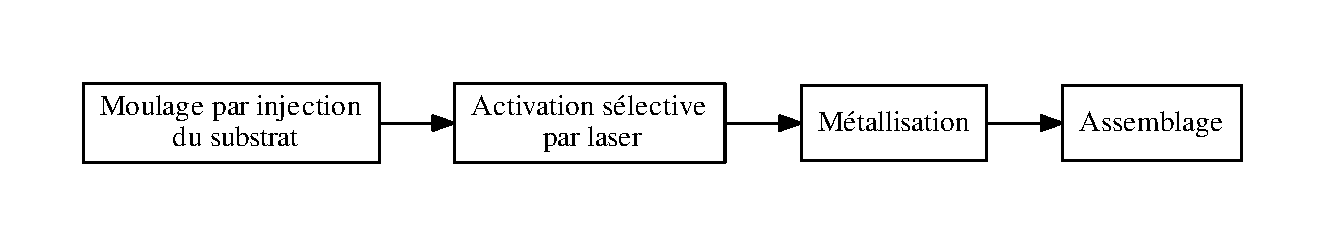
\includegraphics[width=\textwidth]{images/lds_process}
        \caption{Vue d'ensemble du processus \emph{Laser Direct Structuring}}\label{fig:lds-process}
    \end{center}
\end{figure}
Le \gls{lds} est un procédé relativement récent, introduit sur le marché en 2006.
C'est une technologie brevetée de LPKF~Lasers~\&~Electronics~AG en Allemagne, ce qui rend l'utilisation d'une de leur machine obligatoire.
Leur site web\footnote{\url{www.lpkf.com}} est donc une excellente source d'informations pour la conception de pièces utilisant le \gls{lds}.

\subsubsection{Principe de base du procédé}
Le principe général du procédé est visible à la fig.
\ref{fig:lds-process}.
On retrouve donc, dans l'ordre :

\begin{description}
    \item[Injection] La pièce est d'abord moulée par un procédé d'injection standard.
        Le détail de cette étape sort du cadre de ce séminaire.
        On se référera à celui sur l'injection plastique \cite{injection-2013}.

    \item[Activation] Le polymère ayant servi pour l'injection de la pièce a préalablement été dopé avec un composant organométallique qui est activé par le laser en suivant le tracé des pistes voulues.
        Une réaction physique décompose alors ce dopant entre partie métallique et partie organique.
        Les lasers utilisés sont typiquement des lasers infra-rouges d'une longueur d'onde $\lambda = \SI{1000}{\nano\meter}$.
    \item[Métallisation] L'étape de métallisation commence par une étape de nettoyage, afin de faciliter l'accrochage.
        Les pistes sont ensuites construites par déposition de fine couches (environ \SI{5}{\micro\meter}).
        Finalement, un traitement de surface contre l'oxydation est appliqué.
        Ce traitement consiste généralement en une couche de nickel suivie d'une fine couche d'or, mais des traitements spécifiques, à base d'étain ou d'argent sont également possibles.
    \item[Assemblage] Les composants électriques annexes (boutons, connecteurs, etc.) sont soudés sur le \gls{mid}.
        Pendant le prototypage, cette étape est souvent faite à la main, avec un fer à souder.
        Pour la production, si le polymère a une température de fusion suffisament élevée, l'assemblage par \emph{reflow soldering} est possible.
        On peut se référer au séminaire \cite{smd-assembly-2013} pour plus de détails.

\end{description}

% TODO: Section sur l'activation

\subsubsection{Métallisation}
\begin{figure}[h]
    \begin{center}
        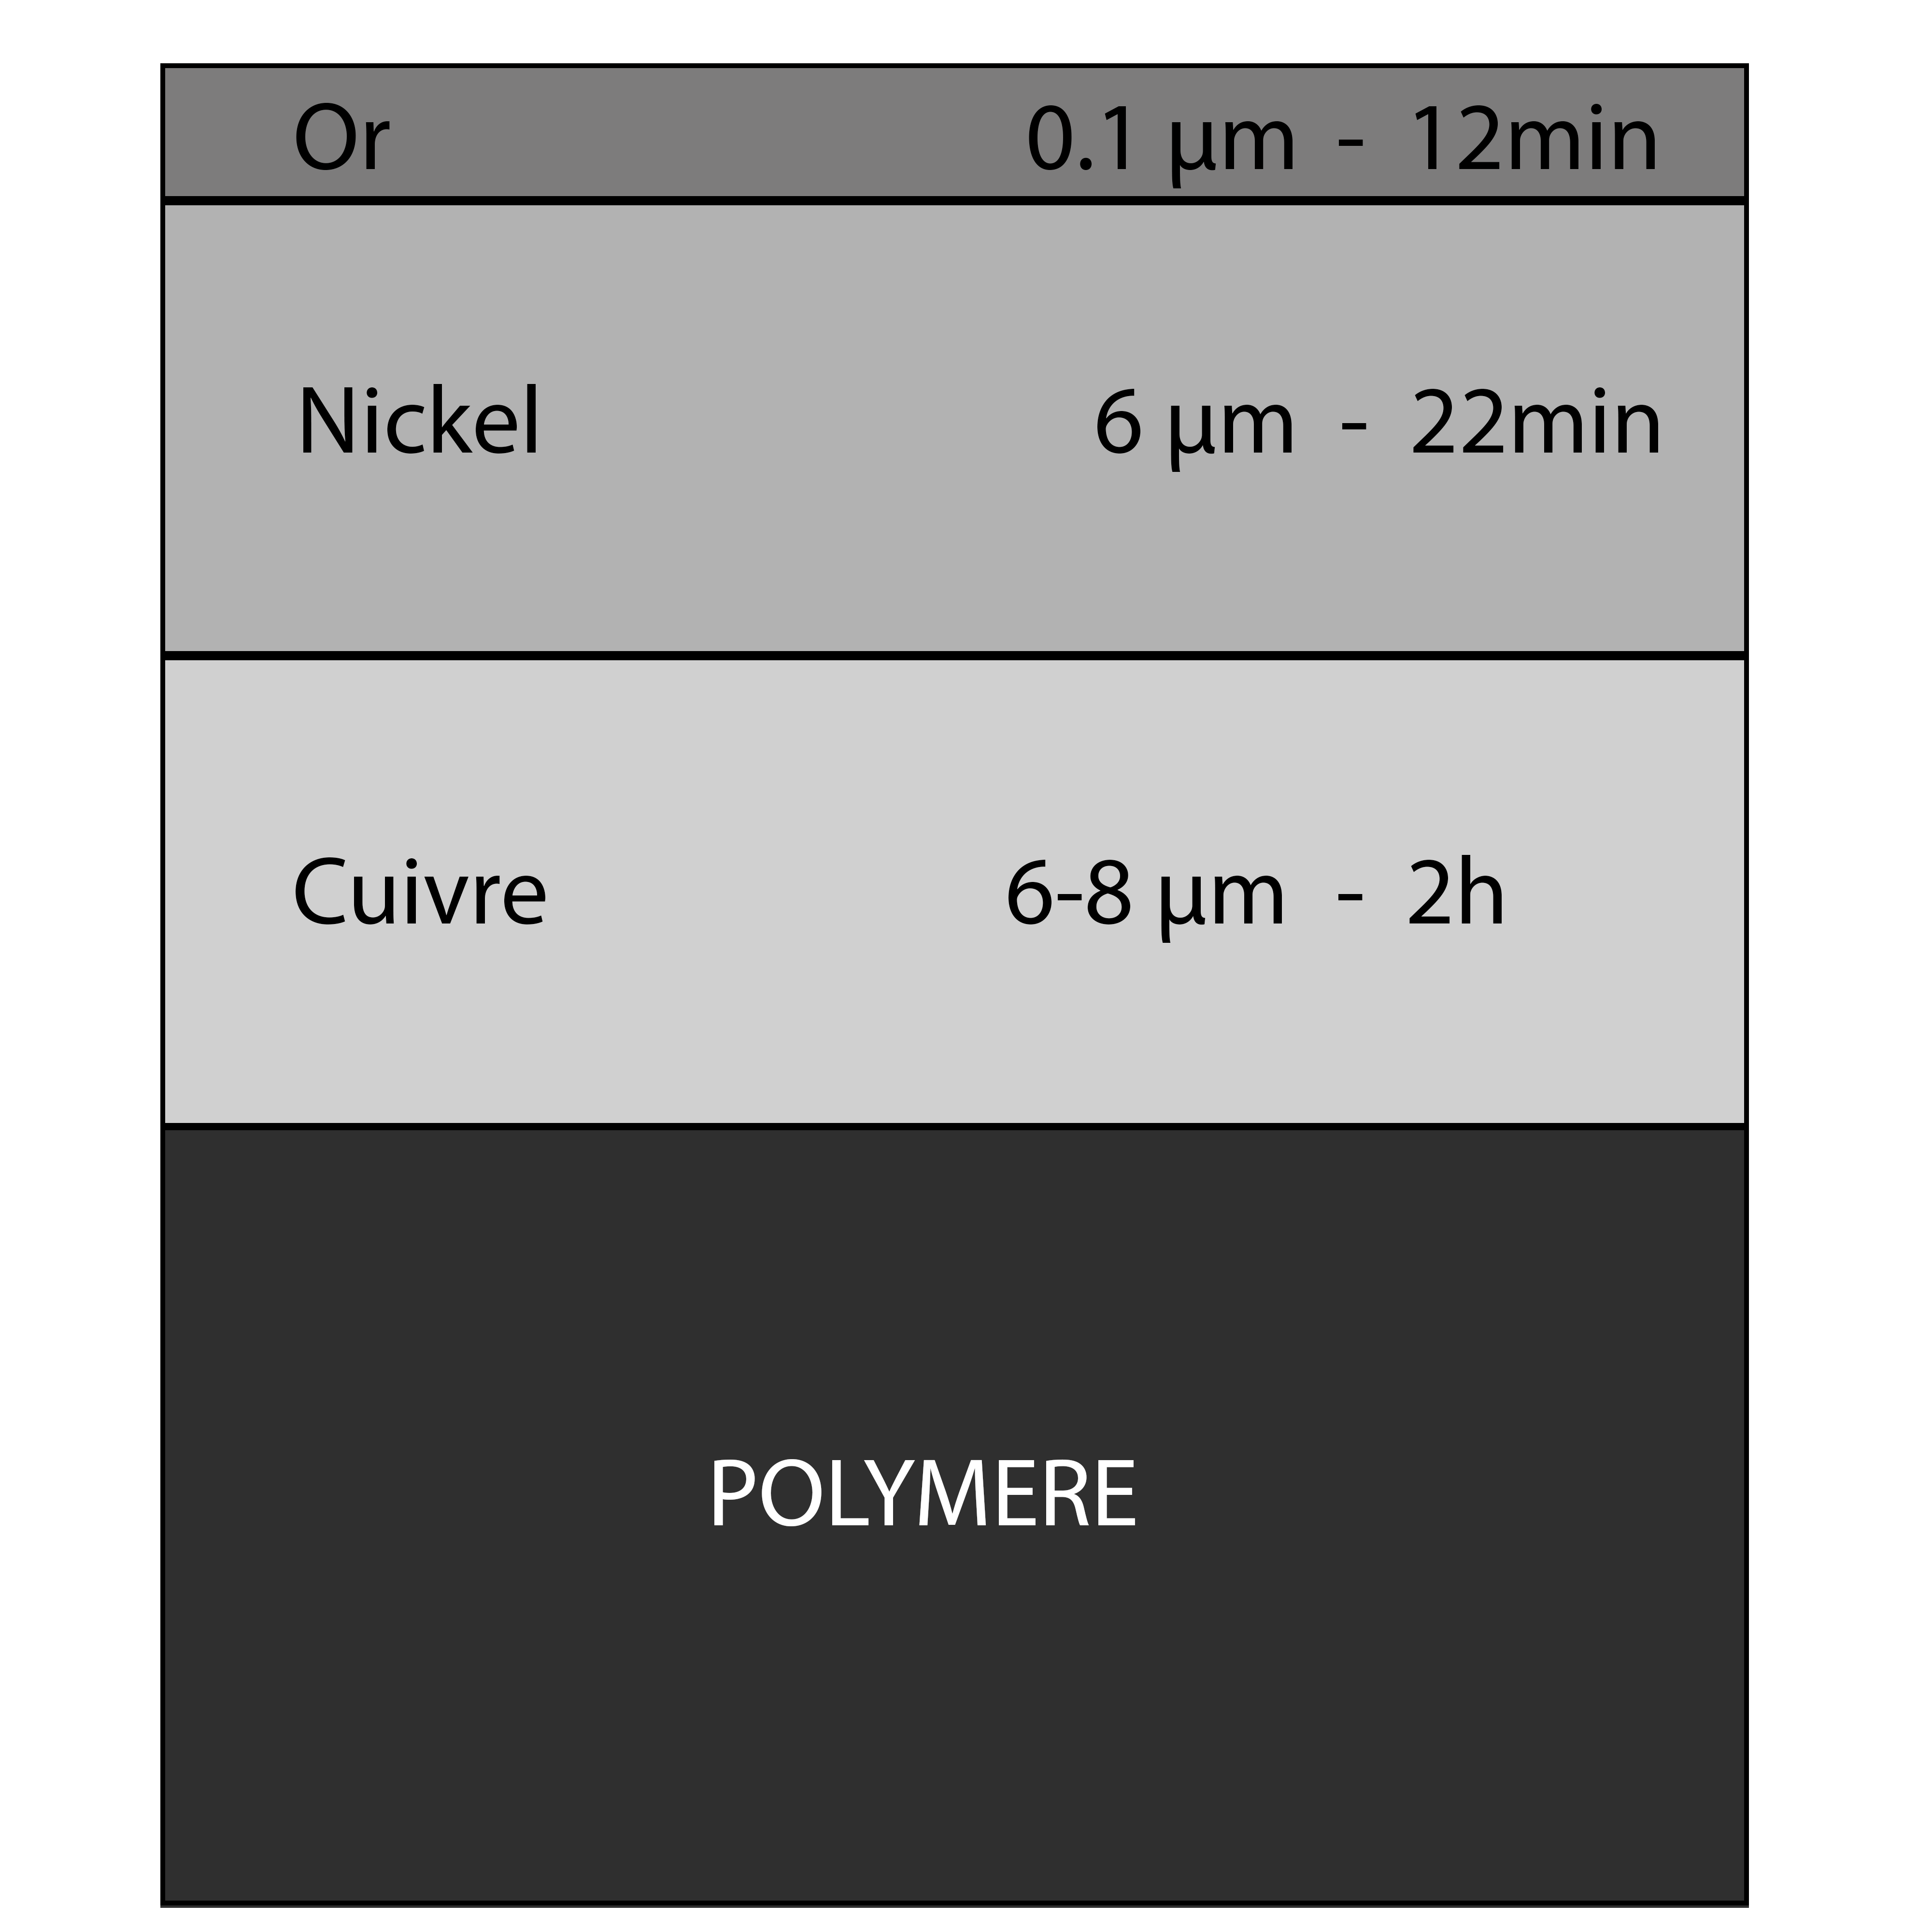
\includegraphics[height=0.3\textheight]{images/CuNiAu}
        \caption{Différentes couches métalliques utilisées en \gls{mid}.
                 L'épaisseur ainsi que le temps nécessaire à la déposition sont également visibles.}
        %\label{fig:lds-process}
    \end{center}
\end{figure}
L'étape de métallisation est celle qui va à proprement parler déposer les pistes sur le polymère.
Afin de garantir le bon fonctionnement de cette étape, un rinçage de la pièce entre chaque bain est effectué, ainsi qu'un séchage à chaud après le dernier bain, afin d'enlever toute trace sur la pièce finale.

Le premier bain de cuivre se fait sans électrolyse, vu qu'aucune piste conductrice n'existe pour le moment.
Dans ce bain, du cuivre va croître autour des atomes de métal présents à la surface du polymère et se liera aux microcavités résultant de l'activation laser.
L'épaisseur maximum atteignable lors de ce premier bain est de 5 à 8 \si{\micro\meter}.

Dans les applications à fort courant, une grande épaisseur de cuivre est souhaitée.
Pour y parvenir, on peut, après le premier bain, faire une déposition éléctrolytique du cuivre.
Pour cela, il faut que toute les pistes soient connectées entre elles en un point.
Si ce n'était pas le cas, il faudrait connecter les pistes une à une à l'éléctrode, ce qui serait long et donc coûteux.
Le point de connexion est généralement placé sur une partie séparable mécaniquement qui est enlevée après la métallisation.

Une fois ce premier bain terminé, une couche de protection contre l'oxydation est appliquée.
En effet une oxydation de la couche de cuivre ruinerait les proprietés électriques du circuit.
Cette couche est généralement composée d'une couche de nickel suivie d'une couche d'or.
Le rôle de cette dernière est d'empêcher l'oxydation de la couche de cuivre, tandis que la couche de nickel sert à empêcher le cuivre de diffuser dans l'or, ce qui détruirait la protection anti-oxydation.

\subsection{Two-shot molding}
Le two-shot molding est un procédé antérieur au \gls{lds} et qui est dans le domaine public.
Il est essentiellement utilisé dans le domaine de l'injection plastique, pour produire des pièces injectées de différentes couleurs, comme des touches de clavier d'ordinateur.
Cette méthode consiste à d'abord mouler les pistes dans un polymère dopé, puis à ``surmouler'' la forme définitive de la pièce autour (fig. \ref{fig:second-shot}).
Finalement, la pièce est métalisée suivant le même procédé que dans le \gls{lds}, mais le cuivre ne se dépose que sur les parties exposées du polymère dopé (fig. \ref{fig:two-shot-metal}).


\begin{figure}[h]
        \centering
        \begin{subfigure}[t]{0.3\textwidth}
                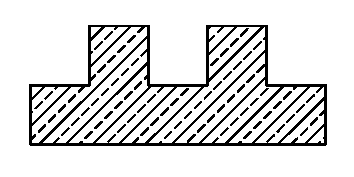
\includegraphics[width=\textwidth]{images/two-shot-example/inner}
                \caption{Injection du polymère dopé.}
                \label{fig:first-shot}
        \end{subfigure}%
        ~ 
        \begin{subfigure}[t]{0.3\textwidth}
                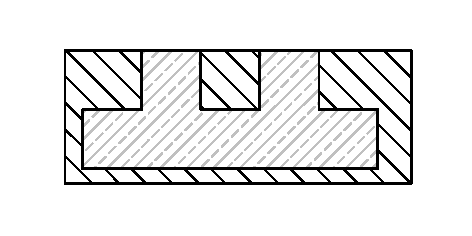
\includegraphics[width=\textwidth]{images/two-shot-example/second_shot}
                \caption{Surmoulage d'un polymère standard.}
                \label{fig:second-shot}
        \end{subfigure}
        ~
        \begin{subfigure}[t]{0.3\textwidth}
                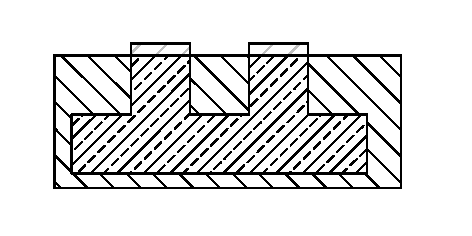
\includegraphics[width=\textwidth]{images/two-shot-example/after_metal}
                \caption{Métallisation.}
                \label{fig:two-shot-metal}
        \end{subfigure}
        \caption{Procédé two-shot}\label{fig:two-shot-process}
\end{figure}


